\section{Actividades con el repositorio GitHub}

\subsection{Creando e inicializando repositorio GitHub}
\begin{itemize}	
	\item Como ya tenemos nuestro repositorio GitHub y además esta clonado e inicializado en nuestra máquina local.
	\item Se realizaron los siguientes comandos en la computadora:
\end{itemize}	

\begin{lstlisting}[language=bash,caption={Creando carpeta de trabajo dentro de nuestro repositorio clonado en mi maquina local}][H]
	$ cd Pweb2-Lab-B
   $ mkdir Lab05-Informe
\end{lstlisting}
\begin{lstlisting}[language=bash,caption={Dirijíéndonos a la carpeta de trabajo}][H]
	$ cd Lab05-Informe
\end{lstlisting}	
\begin{lstlisting}[language=bash,caption={Creando carpetas que contendrán el proyecto e imagenes}][H]
	$ cd Lab05-Informe
   $ mkdir Proyecto_Django/Store
   $ mkdir imagenes
\end{lstlisting}
\begin{lstlisting}[language=bash,caption={Dentro de la carpeta Proyecto_Django/Store, tendremos dos carpetas más Apps/Aplicacion1 y Store}][H]
	$ cd Proyecto_Django/Store
	$ mkdir Apps/Aplicacion1
	$ mkdir Store
\end{lstlisting}

\subsection{Commits}
\begin{itemize}	
	\item A continucación se mostraran capturas de los commits:
\end{itemize}	
\begin{figure}[H]
	\centering
	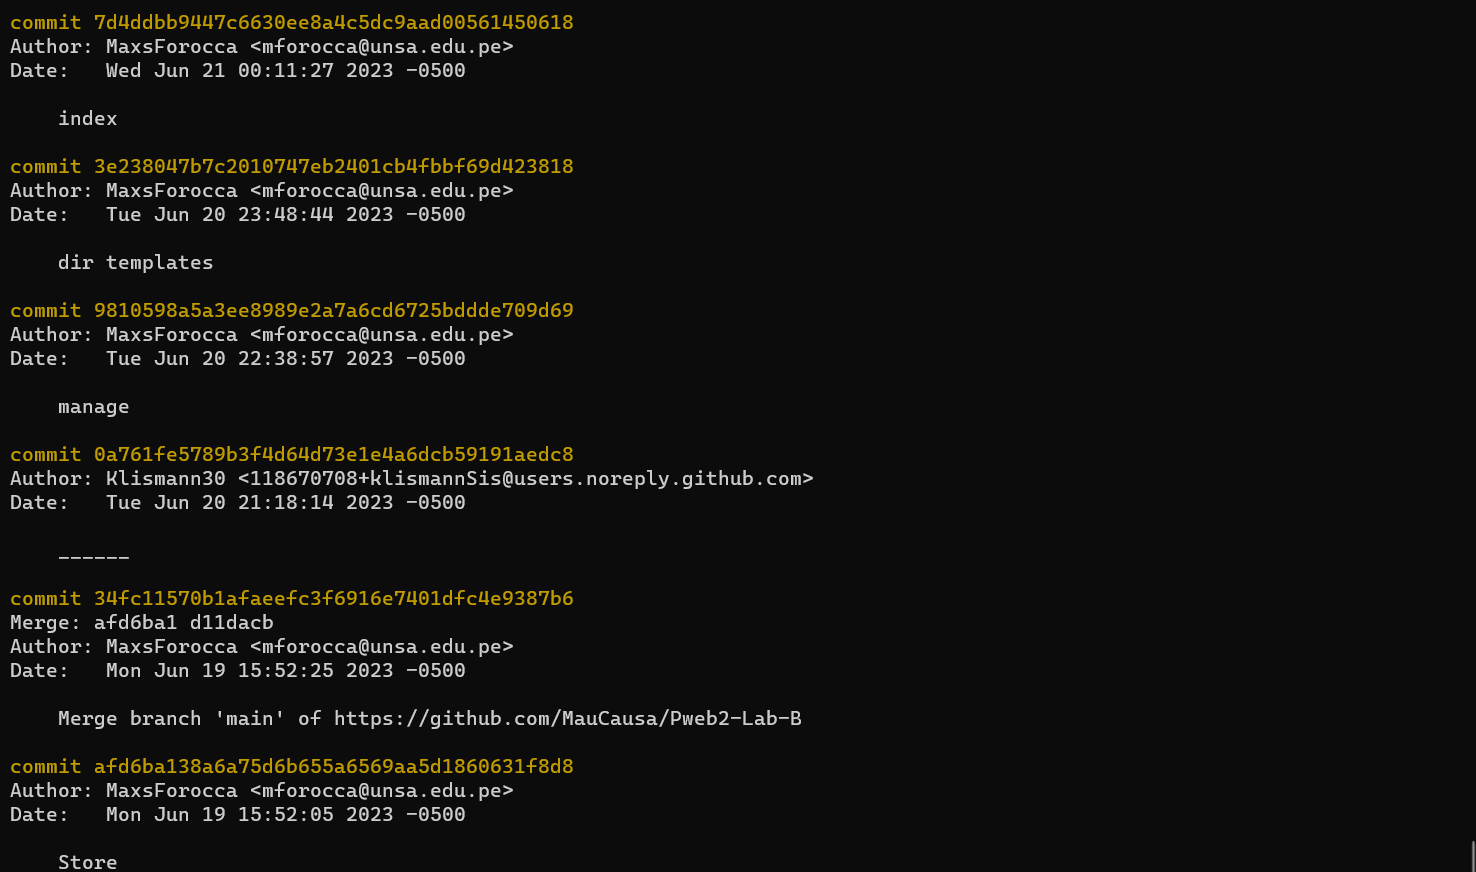
\includegraphics[width=0.8\textwidth,keepaspectratio]{img/commits1.png}
	%\includesvg{img/automata.svg}
	%\label{img:mot2}
	%\caption{Product backlog.}
\end{figure}
\begin{figure}[H]
	\centering
	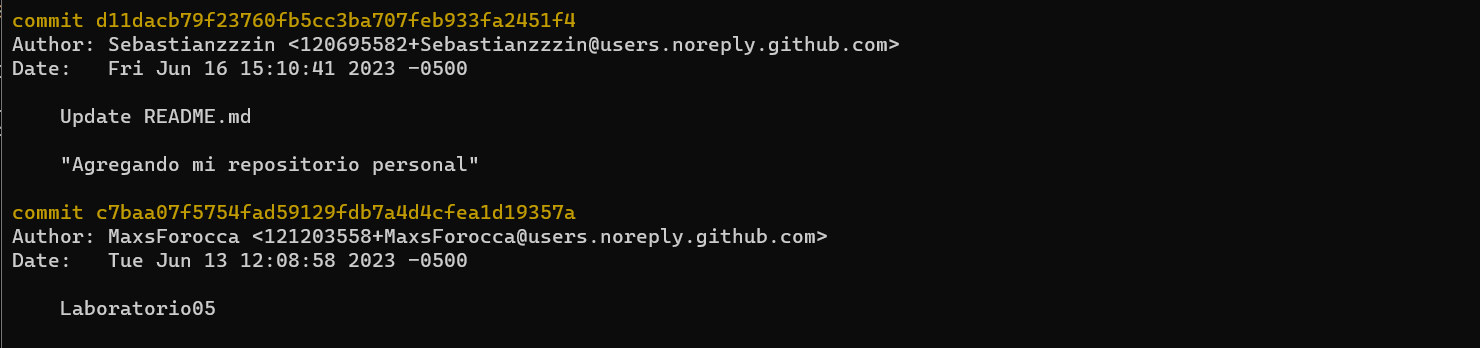
\includegraphics[width=0.8\textwidth,keepaspectratio]{img/commits2.png}
	%\includesvg{img/automata.svg}
	%\label{img:mot2}
	%\caption{Product backlog.}
\end{figure}
\begin{itemize}	
	\item Todo esto serían los archivos y orden de nuestro laboratorio 05:
\end{itemize}	
\begin{figure}[H]
	\centering
	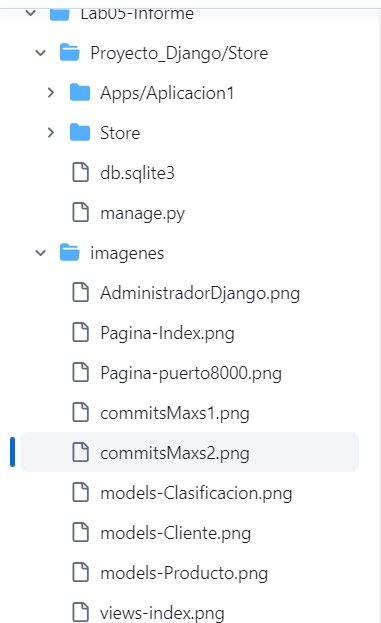
\includegraphics[width=0.8\textwidth,keepaspectratio]{img/estructura3.jpg}
	%\includesvg{img/automata.svg}
	%\label{img:mot2}
	%\caption{Product backlog.}
\end{figure}
\subsection{Capturas importantes del desarrollo del laboratorio 05}
\begin{itemize}	
	\item Administrador Django:
\end{itemize}	
\begin{figure}[H]
	\centering
	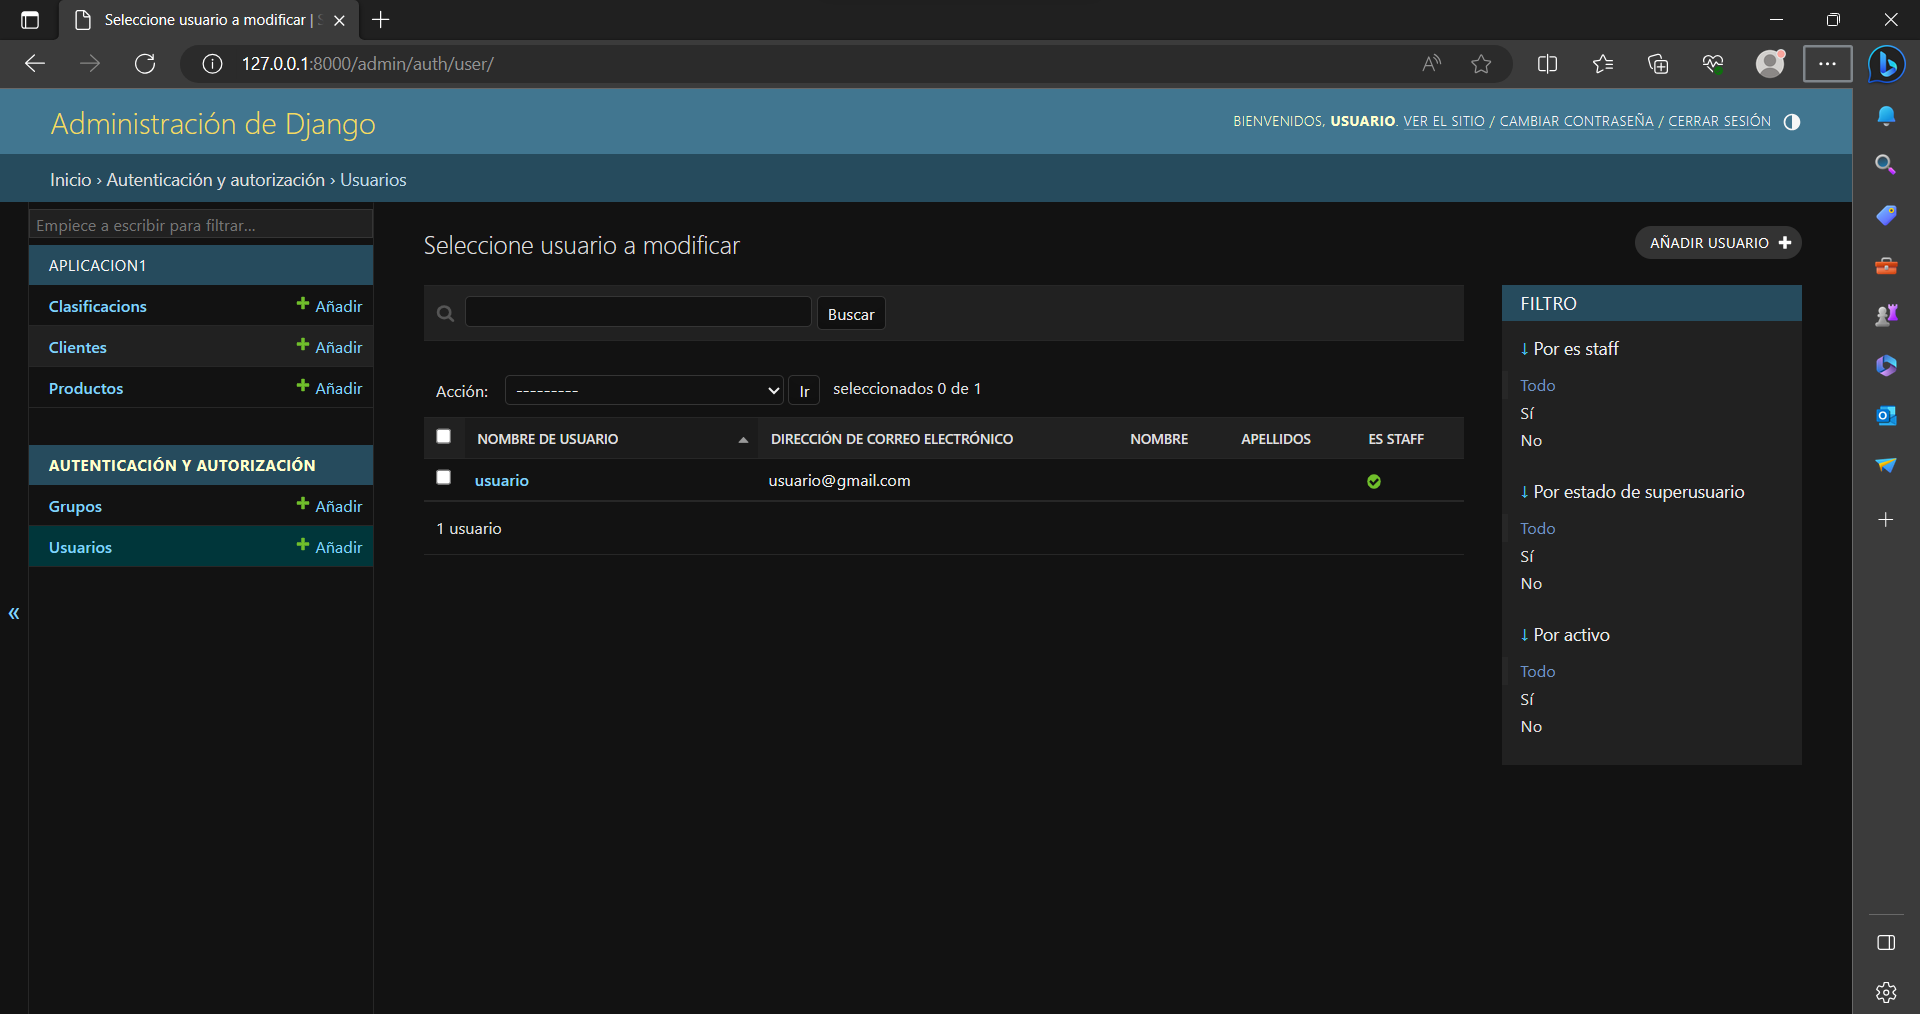
\includegraphics[width=0.8\textwidth,keepaspectratio]{img/AdministradorDjango.png}
	%\includesvg{img/automata.svg}
	%\label{img:mot2}
	%\caption{Product backlog.}
\end{figure}
\begin{itemize}	
	\item Página index:
\end{itemize}	
\begin{figure}[H]
	\centering
	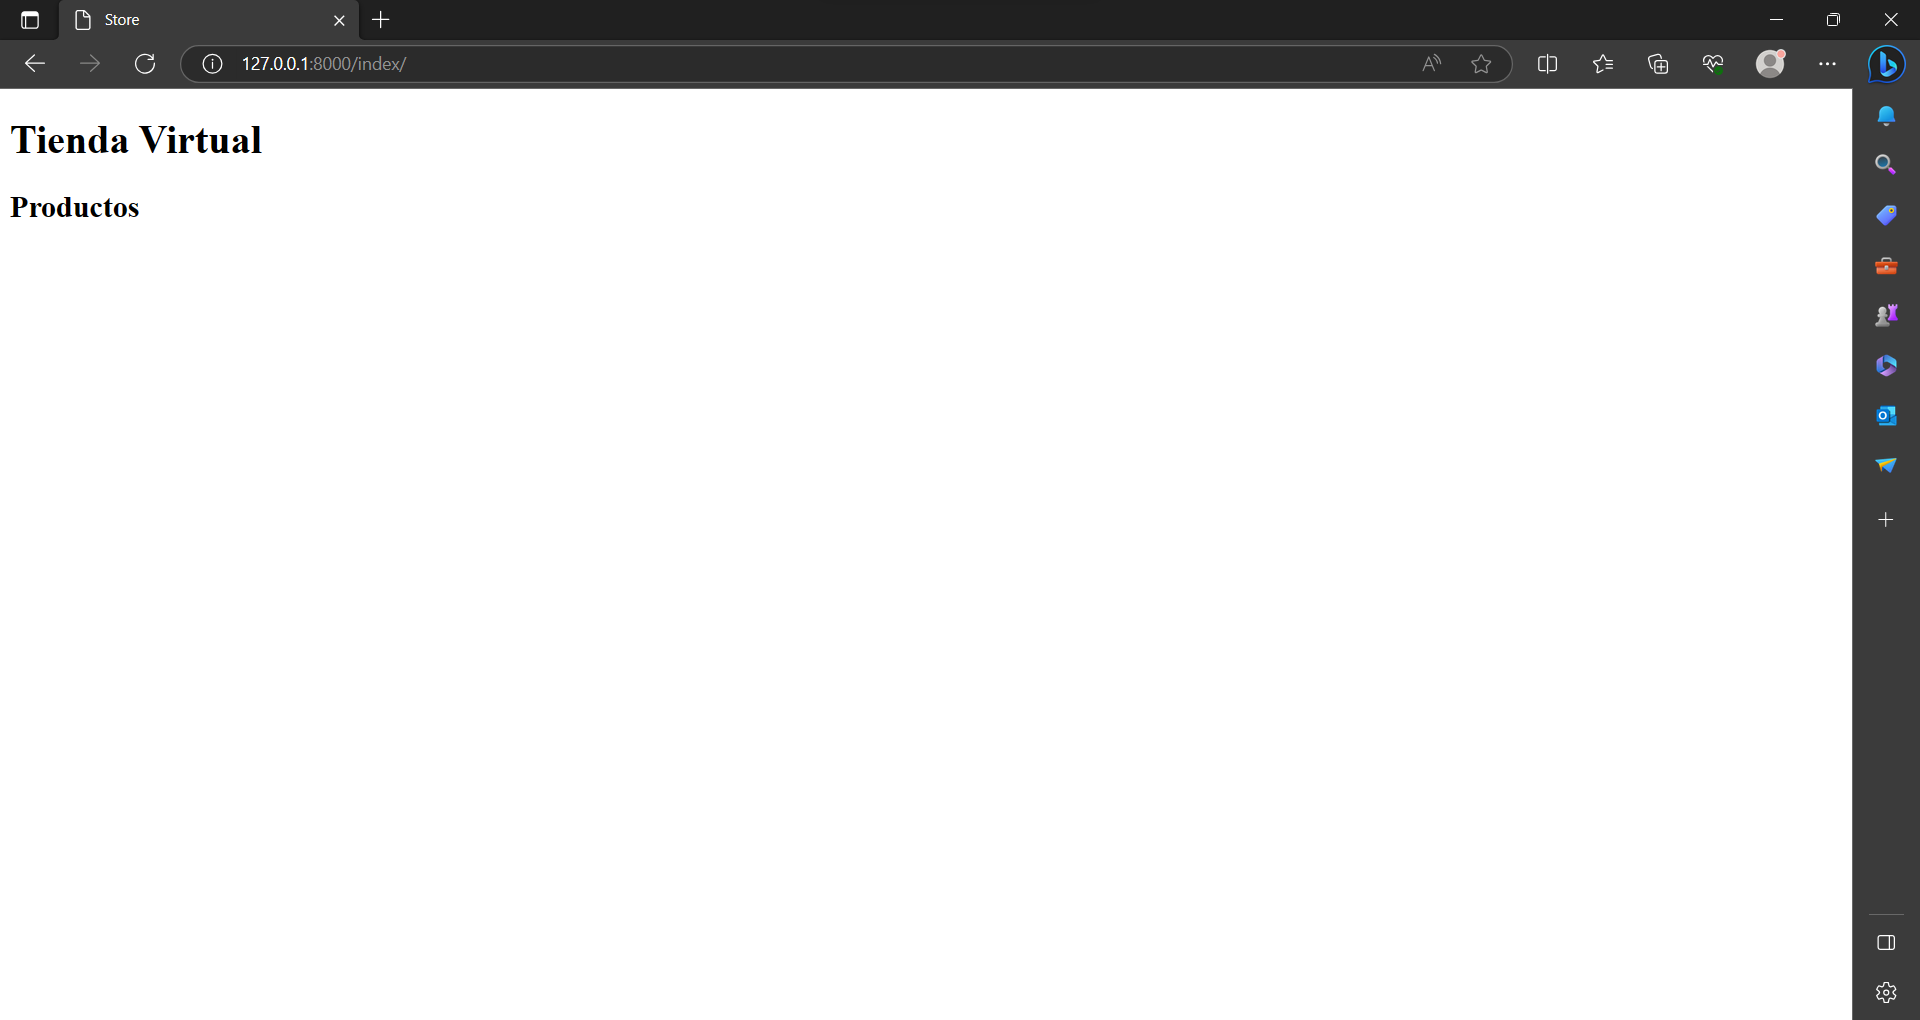
\includegraphics[width=0.8\textwidth,keepaspectratio]{img/Pagina-Index.png}
	%\includesvg{img/automata.svg}
	%\label{img:mot2}
	%\caption{Product backlog.}
\end{figure}
\begin{itemize}	
	\item Página puerto 8000:
\end{itemize}	
\begin{figure}[H]
	\centering
	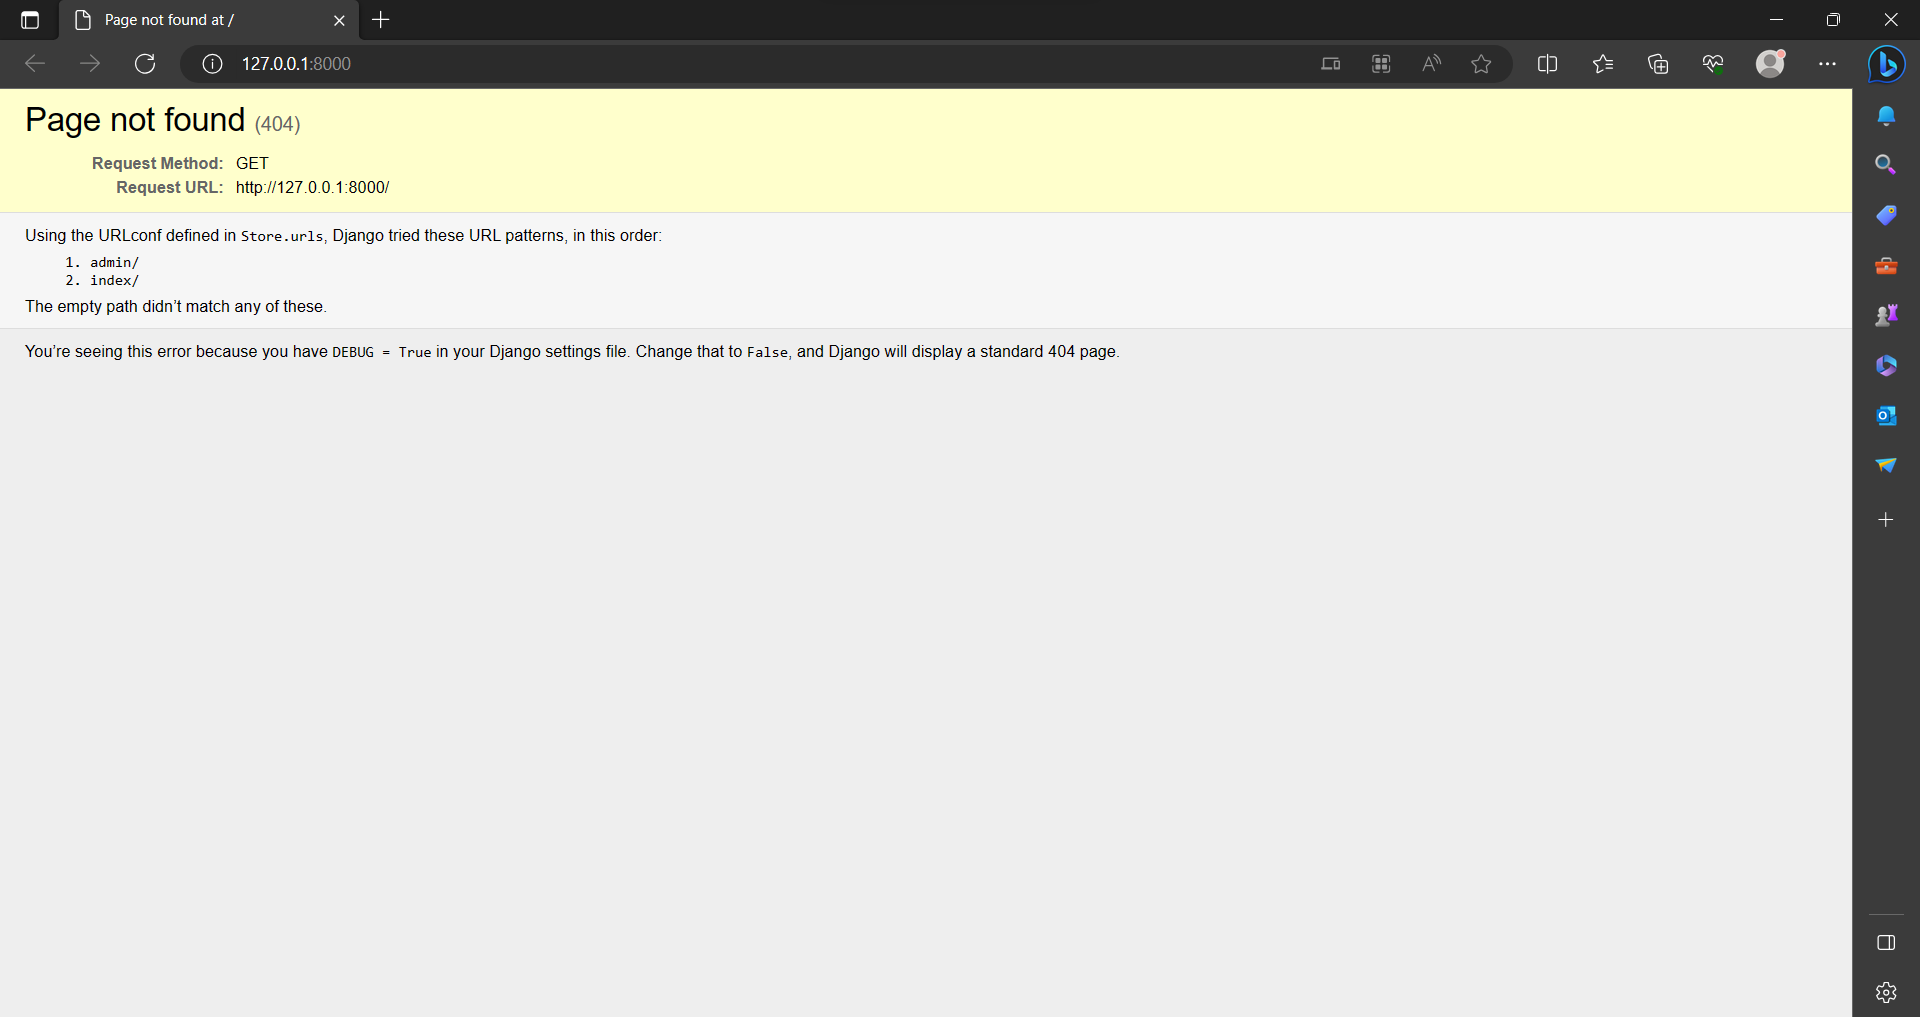
\includegraphics[width=0.8\textwidth,keepaspectratio]{img/Pagina-puerto8000.png}
	%\includesvg{img/automata.svg}
	%\label{img:mot2}
	%\caption{Product backlog.}
\end{figure}
\begin{itemize}	
	\item Models - clasificación:
\end{itemize}	
\begin{figure}[H]
	\centering
	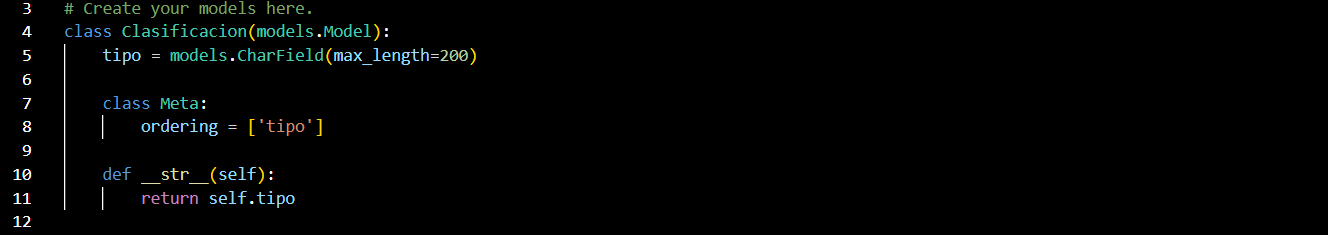
\includegraphics[width=0.8\textwidth,keepaspectratio]{img/models-Clasificacion.png}
	%\includesvg{img/automata.svg}
	%\label{img:mot2}
	%\caption{Product backlog.}
\end{figure}
\begin{itemize}	
	\item Models - clientes:
\end{itemize}	
\begin{figure}[H]
	\centering
	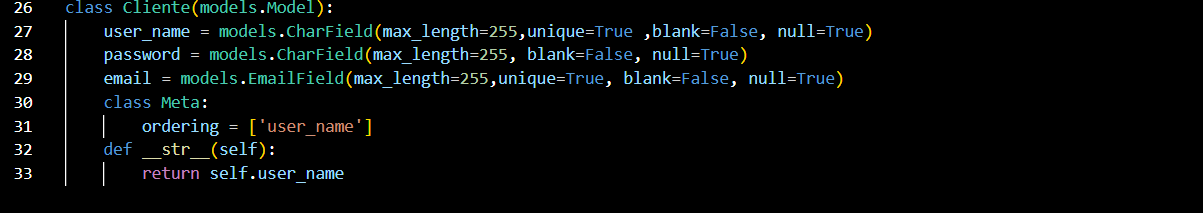
\includegraphics[width=0.8\textwidth,keepaspectratio]{img/models-Cliente.png}
	%\includesvg{img/automata.svg}
	%\label{img:mot2}
	%\caption{Product backlog.}
\end{figure}
\begin{itemize}	
	\item Models - producto:
\end{itemize}	
\begin{figure}[H]
	\centering
	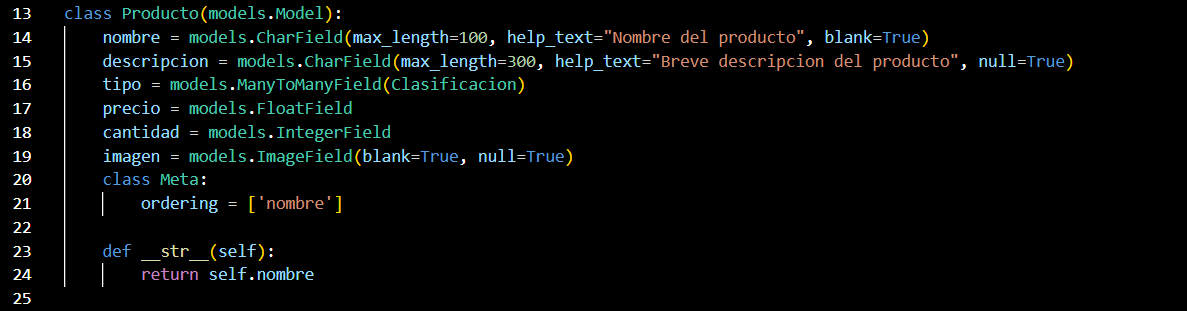
\includegraphics[width=0.8\textwidth,keepaspectratio]{img/models-Producto.png}
	%\includesvg{img/automata.svg}
	%\label{img:mot2}
	%\caption{Product backlog.}
\end{figure}
\begin{itemize}	
	\item View - index:
\end{itemize}	
\begin{figure}[H]
	\centering
	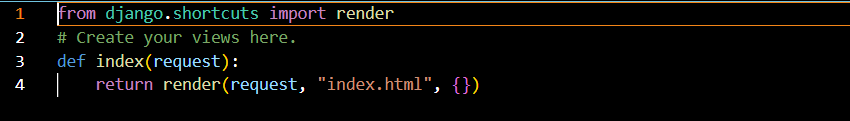
\includegraphics[width=0.8\textwidth,keepaspectratio]{img/views-index.png}
	%\includesvg{img/automata.svg}
	%\label{img:mot2}
	%\caption{Product backlog.}
\end{figure}
\subsection{Estructura de laboratorio 05}
\begin{itemize}	
	\item El contenido que se entrega del informe del laboratorio 05 es el siguiente:
\end{itemize}

\begin{lstlisting}[style=ascii-tree]
	Lab05-Informe/
   |--- informe-latex
	|--- contenido
   |   |--- actividades.tex
   |   |--- caratula.tex
   |   |--- github.tex
   |   |--- materiales.tex
   |   |--- preguntas.tex
   |   |--- referencia.tex
   |   |--- rubrica.tex
   |   |--- tarea.tex
	|--- img
   |   |--- logo_abet.png
   |   |--- logo_episunsa.png
   |   |--- logo_unsa.jpg
   |   |--- AdministradorDjango.png
   |   |--- commits1.png
   |   |--- commits2.png
   |   |--- estructura3.jpg
   |   |--- models-Clasificacion.png
   |   |--- models-Cliente.png
   |   |--- models-Producto.png
   |   |--- Pagina-Index.png
   |   |--- Pagina-puerto8000.png
   |   |--- views-idex.png
   |--- pweb2_lab05_aalfonso.pdf    
   |--- main.tex
\end{lstlisting}    